\chapter{Periodograms}
\label{ch:axions-periodograms}
The space of possible axion-induced signals is spanned by their amplitude (the strength of the coupling) and their frequency (the axion mass). The problem is, therefore, naturally set in the frequency domain. The analysis was performed in two steps. First, the measurements were transformed from the time domain into the frequency one by evaluating the periodogram of the time series. In the second step the periodogram was checked for statistically significant signals.

In this chapter we introduce the statistical methods used in the analysis. We start by defining the periodogram, which serves as a transition from time to the frequency space, natural for looking for oscillations. Next, we proceed to discuss the statistical properties of the periodogram.

% For the sake of pedagogy we will discuss the methodology on a simple example.



\section{Definition of the periodogram}
A \emph{periodogram} is an estimator of the power spectrum. It has been proposed as the preferred way to treat periodic signals as early as 1898~\cite{Schuster1898}. In its simplest form it is the squared magnitude of the discrete Fourier transform, which, however, is only possible for evenly sampled series. Lomb and Scargle have independently described a method to construct a statistically well-behaving periodogram for non-uniformly sampled data with unequal error-bars: the Least Squares Spectral Analysis (LSSA)~\cite{Scargle1982}. It is also known as the Lomb-Scargle periodogram.

% Many packages readily offer procedures to evaluate Lomb--Scargle periodograms~\cite{scipy,astropy}. They could not, however, be used directly as the analysis deviated in details from the standard procedure. We had to take a low--level approach, instead.

\begin{figure}
  \centering 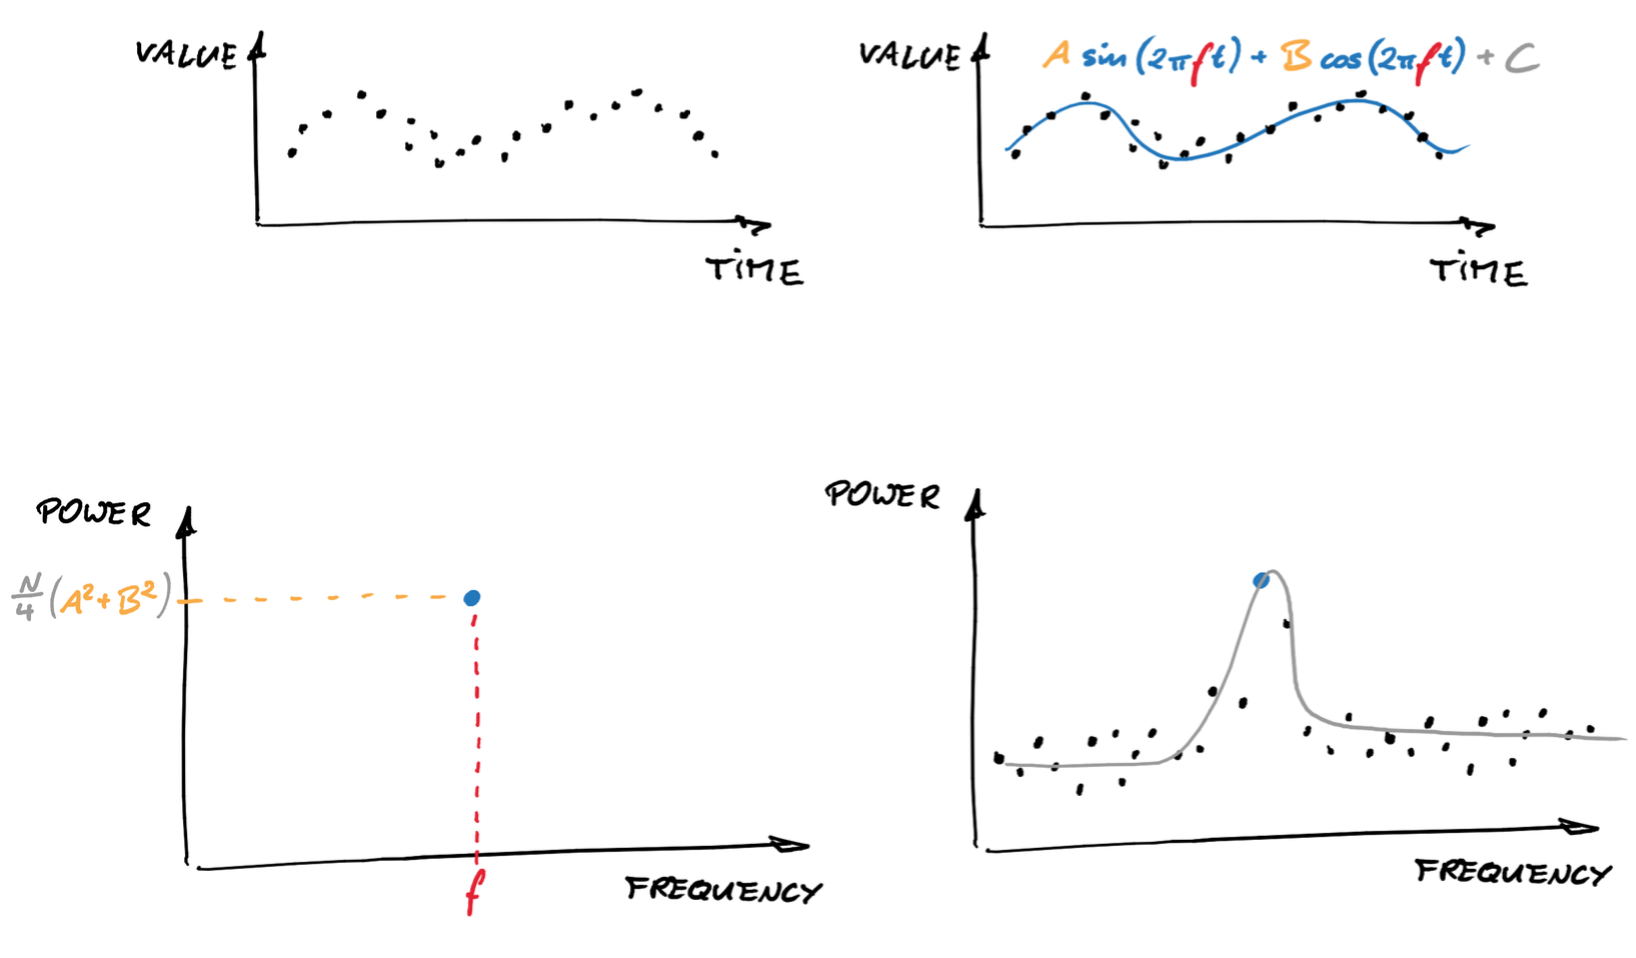
\includegraphics[width=\linewidth]{gfx/axions/LSSA}
  \caption{The LSSA periodogram, a function of frequency, is constructed by performing a linear least--squares fit at each of those frequencies.}
  \label{fig:LSSA_overview}
\end{figure}

In order to evaluate the LSSA periodogram at a circular frequency $\omega$, one performs a linear least-squares fit (hence the name) to the data with a function
\marginpar{LSSA, in contrast to the fast Fourier transform (FFT), does not require windowing, because it is explicitly phase-aware.}
\begin{equation}
  A\,\mathrm{cos}(\omega t) + B\,\mathrm{sin}(\omega t) + C \ ,
\end{equation}
where $A$, $B$ and $C$ are free parameters. The estimator of power $P(\omega)$ is then defined as
\begin{equation}
  P(\omega) := \frac{N}{4} \, \left( A^2 + B^2 \right) \ ,
\end{equation}
where $N$ is the number of data points. Different normalisations may be used.
\marginpar{The noise bed is flat part of periodogram due to random noise. If there is a signal, it is said to ,,rise out of the noise bed''.}
We use the one of \cite{Scargle1982}, where the height of $\sqrt{P(\omega)}$ at the noise bed corresponds numerically to the size of the error-bars squared, if they are all equal. A graphical overview of the method is shown in Fig.\,\ref{fig:LSSA_overview}. Throughout the analysis the figure of merit is either the power $P(\omega)$ or, interchangeably, its square root---amplitude. The latter has conveniently the same unit as the time series.

\begin{figure}
  \centering 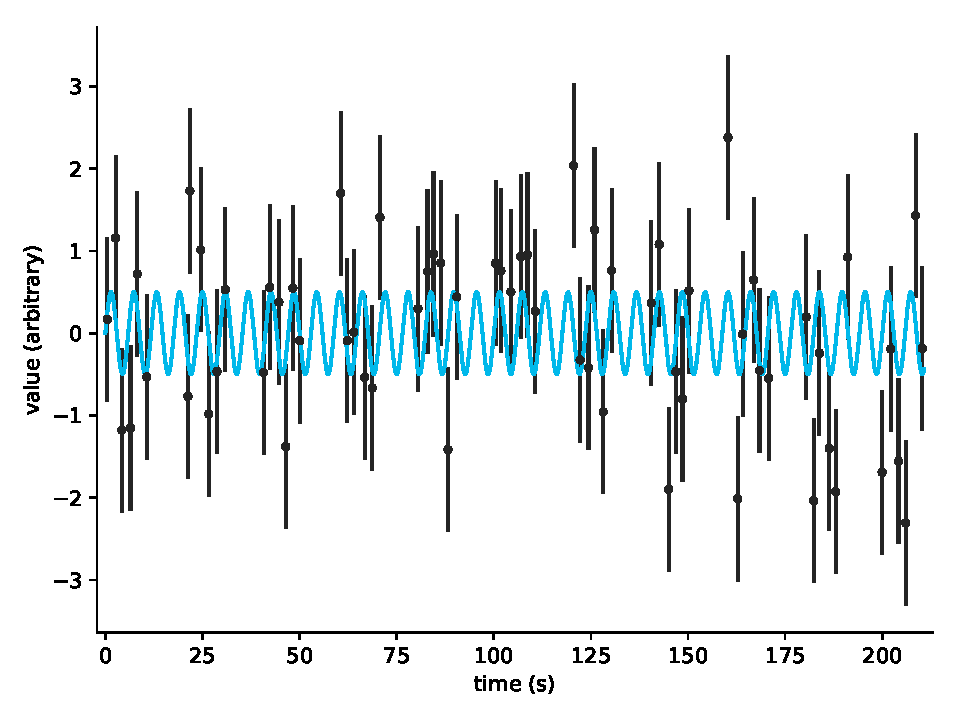
\includegraphics[width=0.8\linewidth]{gfx/axions/basic_signal.pdf}
  \caption{A simple signal generated just for the purpose for explaining the general scheme of periodogram analysis. A harmonic signal (blue) was used to generate unevenly spaced data points (black) with unequal error bars. Each point was drawn from a normal distribution centred at the blue curve and width corresponding to its error bar.}
  \label{fig:basic_signal}
\end{figure}

We will now follow an analysis of a toy time series, shown in Fig.\,\ref{fig:basic_signal}. The time series are simulated measurements of an oscillating signal of the frequency \SI{0.17}{\hertz}. The series has already some properties of the actual dataset. The measurements are not equally spaced. They are randomly grouped in 10--second long bunches, aronud 20 seconds apart. Inside a bunch a ,,measurement'' is taken every 2~seconds with a \SI{0.3}{\second} jitter. The length of each measurement is 1~second with a \SI{0.1}{\second} jitter. The error-bars are all size one in the arbitrary unit. An oscillating signal with an amplitude 0.7 and frequency \SI{0.17}{\hertz}. Each measurement averages the signal over its duration.

The immediate question arising when evaluating the LSSA periodogram is: for which frequencies to evaluate the power? In case of evenly-spaced series the upper limit is the Nyquist frequency, equal to the half of the sampling rate~\cite{Shannon1949}. It is not the case when the sampling is not uniform. In practice, we can expect little sensitivity to oscillations faster than the period over which each signal is averaged, \SI{1}{\second} in the example. On the low side the limit is zero, which corresponds to the constant offset (a least-squares fit of a horizontal line, which is equivalent to calculating the average of the points). The value of the periodogram at zero is often not plotted.

\begin{figure}
  \centering 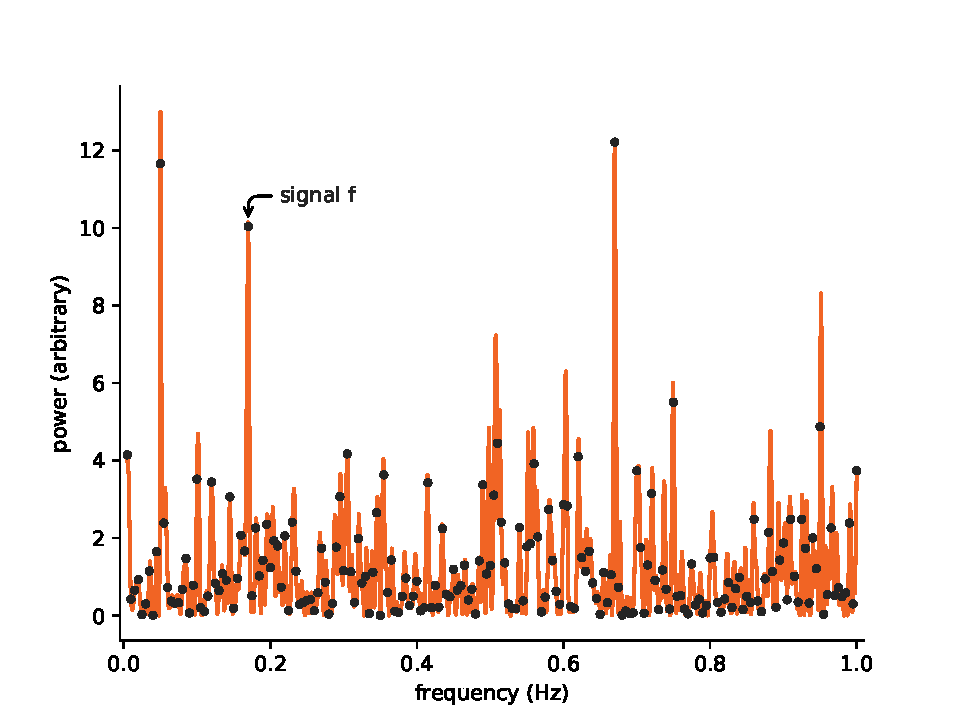
\includegraphics[width=0.8\linewidth]{gfx/axions/basic_periodogram.pdf}
  \caption{Two periodograms of the time series in Fig.\,\ref{fig:basic_signal}. One evaluated at frequencies a spectral resolution apart (black dots), and one evaluated a thousand times more densely (the orange line). As no structure on a scale finer the spectral resolution can be accessed, the orange line simply ,,connects'' the black dots.}
  \label{fig:basic_periodogram}
\end{figure}

When choosing the spacing between the frequencies, the \emph{spectral resolution} is considered, defined as the inverse span of the dataset. It roughly defines the minimal frequency difference between two signals that is distinguishable. In Fig.\,\ref{fig:basic_periodogram} there are two periodograms: evaluated at frequencies a spectral resolution apart (black dots), and one evaluated a thousand times more densely (the orange line). As no structure on a scale finer the spectral resolution can be accessed, the orange line simply ,,connects'' the black dots smoothly.

\begin{figure}
  \centering 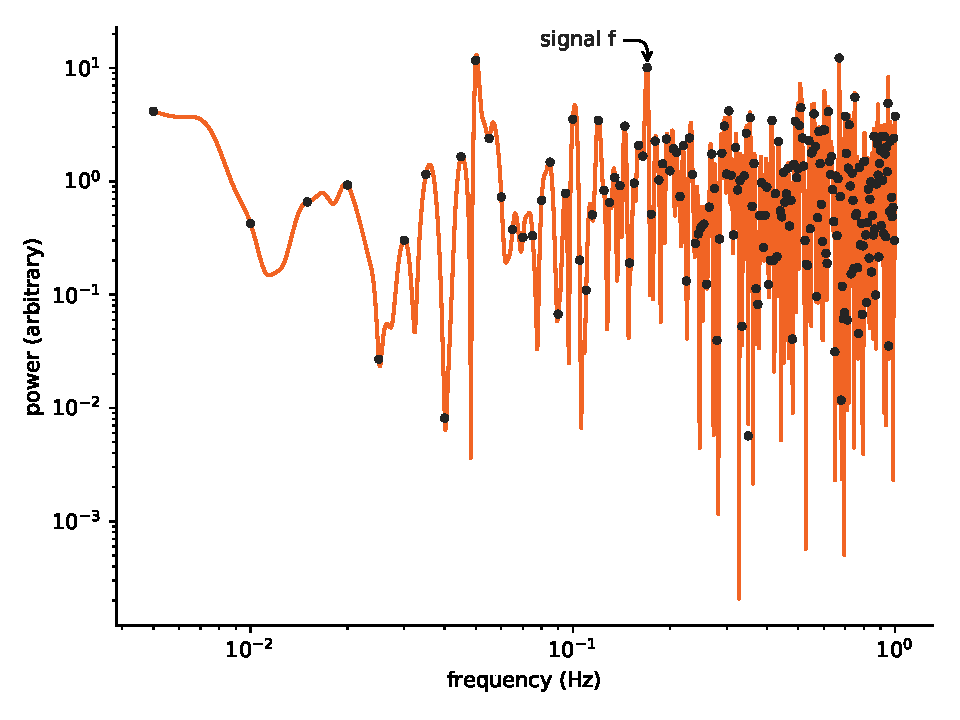
\includegraphics[width=0.8\linewidth]{gfx/axions/basic_periodogram_loglog.pdf}
  \caption{The two periodograms as in Fig.\,\ref{fig:basic_periodogram} plotted on a log-log scale. The range of frequencies where the periodogram is evaluated is extended. The amplitude of the noise appears to be increasing with frequency, but it is not true. Only the density of the evaluated points increases, making the extreme deviations more pronounce.}
  \label{fig:basic_periodogram_loglog}
\end{figure}

Figure~\ref{fig:basic_periodogram_loglog} shows the same two periodograms in a log-log scale. Additionally, the range of frequencies where the periodogram is evaluated has been extended to show its behaviour in the extremes. The logarithmic scale, albeit useful when the potential signals span orders of magnitude in both frequency and amplitude, can lead to misunderstandings. Specifically, the noise appears to increase in amplitude with frequency, but the effect is purely cognitive. The spacing of the points is linear, so on a logarithmic scale the density of points increases for high amplitudes, making the extreme deviations more likely to appear in the same plot area, despite the noise amplitude being the same.

An oscillation in the time series produces a peak in the periodogram. The position of the peak is the frequency of the oscillation, the width corresponds to the coherence of the signal. However, there are the periodogram many peaks besides the one corresponding to the oscillation used when generating the data. Some are even bigger and there are many smaller ones. In the next section we will consider what, besides an oscillating signal, may give rise to a peak. Most importantly a way of determining whether a peak is caused by an oscillation is presented.




\section{A null hypothesis test}
Once the periodogram of a time series is calculated, one would like to know whether it contains a signal signature. For a periodic signal this would be a peak. In our case, the really interesting statement is the answer to the question:

\begin{center}
  \emph{How likely is it that the highest peak in the periodogram is not only a random fluctuation?}
\end{center}

% We are, in fact, interested in the \emph{least likely} peak, which may not be the same as the highest one. For clarity we are going to be first considering the highest peak, and explain the difference later.

This question has already been stated by Scargle~\cite{Scargle1982}. In this section we will be largely following the reasoning he presented, with few important differences.

To describe the question mathematically, let us denote the time series under consideration by $D$. The periodogram is then a set of $P^D(\omega_i)$, depicted with a black line in Fig.\,\ref{fig:basic_detection}. In a uniformly sampled case with equal error bars $P^D(\omega_i)$ is equally exponentially distributed, for those frequencies where no signal is present~\cite{Scargle1982}. In our, more complicated, case the distribution can be generated by a Monte Carlo (MC) simulation in the following way: a new signal is generated, keeping the time position and the size of the error bars, but with no underlying signal present (the null hypothesis $H_0$). The value for each simulated measurement is simply drawn from a gaussian distribution with the width corresponding to the size of the error bar. Then, the periodogram of the generated time series is calculated. This is repeated, yielding a set of periodograms, which are used to estimate the probability density function (PDF) of $P(\omega_i)$ for each $i$. The PDF for $\omega = \SI{0.17}{\hertz}$ is depicted is the right-hand side of~Fig.\,\ref{fig:basic_detection}. In the left-hand side of this figure the 1-, 2- and 3$\upsigma$ bands of the $P(\omega_i)$ PDFs are depicted in shades of green. For uniformly sampled data with equal error bars all PDFs would be the same and the $upsigma$ bands flat~\cite{Scargle1982}. In our case structures appear, despite absolutely no signal being present in the generated time series.

\begin{figure}
  \centering 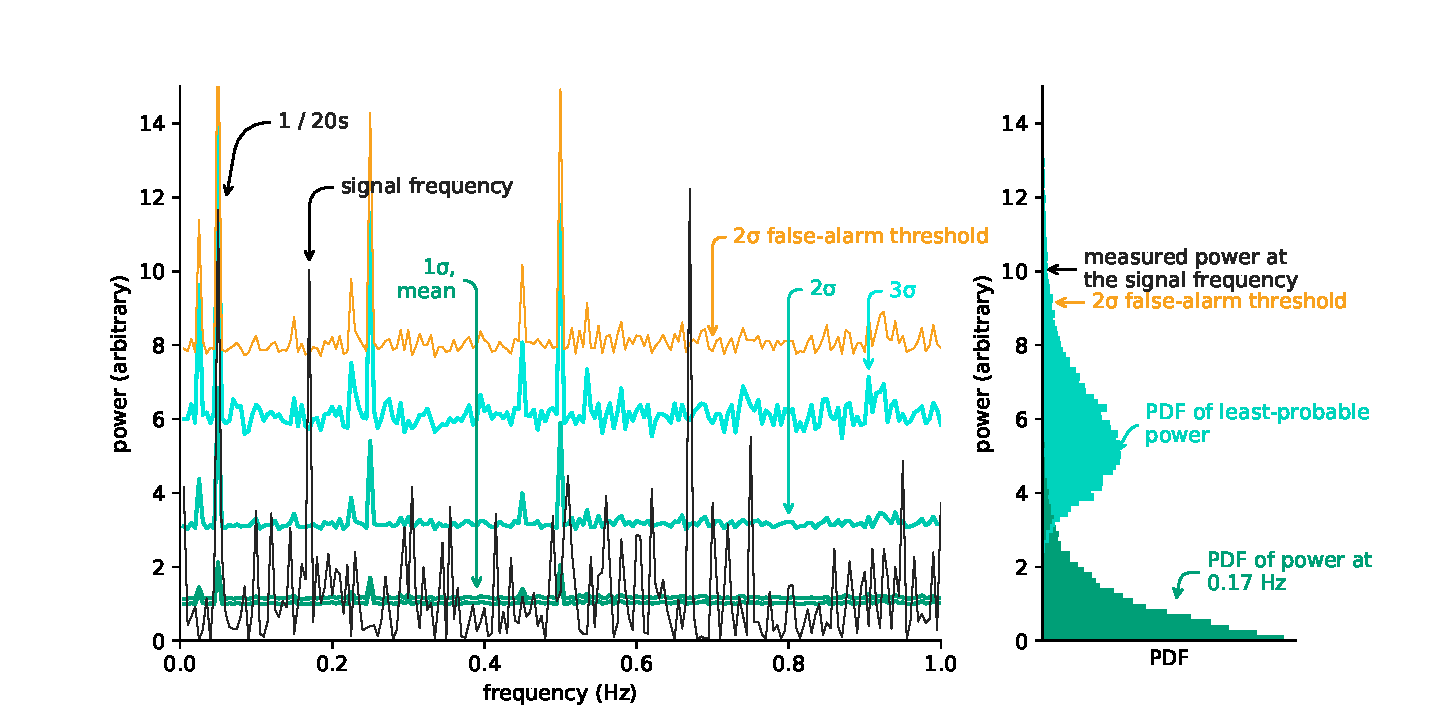
\includegraphics[width=\linewidth]{gfx/axions/basic_detection.pdf}
  \caption{Left-hand side: Juxtaposition of the periodogram of the toy time series (black) and the periodogram PDF under the null hypothesis. For the latter the average and 1-, 2- and 3$\upsigma$ bands are depicted. Right-hand side: Aligned with the plot to the left, two PDFs are depicted: the one of the power at \SI{0.17}{\hertz} (the frequency of the signal put into the toy time-series) and the one of the globally least-probable power (across all frequencies).}
  \label{fig:basic_detection}
\end{figure}

The structures in the $P(\omega_i)$ PDFs are caused solely by the non-uniformity in sampling and in the sizes of the error bars. In particular, we can identify a very large expected rise in power at \SI{0.05}{\hertz}, corresponding exactly to the inverse spacing between the bunching (\SI{20}{\hertz}) introduced in the toy measurement. A peak is expected in the periodogram to appear at this point, even when there is no significant oscillation of this frequency. This is the reason why the most significant peak should be sought, rather than simply the highest. This conclusion makes the presented reasoning different from the one of Scargle~\cite{Scargle1982}.

%We will be using the Cumulative Density Function (CDF) formalism.
We denote the cumulative density function (CDF) of the power estimator at the $i$th frequency as $F_i(z)$ ($z$ would be the power estimated at frequency $\omega_i$). In an evenly sampled, signal-free case it has a functional form
\begin{equation}
  F_i(z) = 1 - e^{-z} \ .
\end{equation}
In our case it can be estimated from the MC simulations. Then the $i$th p-value is directly
\begin{equation} \label{eq:local_p_value}
  p_i = 1 - F_i\left( P^D(\omega_i) \right) \ .
\end{equation}
\marginpar{P-value is the the probability that at least this much power would arise only as a result of a random fluctuation.}
The most significant peak is the one with the lowest p-value. Yet, in the example signal there are 15 peaks with p-values on a 2$\upsigma$ level, much more than expected (a 2$\upsigma$ event is a five-in-a-hundred one). This is due to the so-called \emph{look-elsewhere effect}, best explained as follows: one-in-a-thousand event in a system is not a surprise, if it occurs in one of a thousand different systems. By looking at the Fig.\,\ref{fig:basic_detection} and comparing the periodogram of the signal with the $\upsigma$ bands, one essentially performs many, as many as the number of frequencies, largely independent statistical tests, cherry-picking among them the most significant peaks. The p-values $p_i$ are called \emph{local}, because they only measure the local significance at $\omega_i$.

There is an another way of understanding this phenomenon. The height of the most significant peak is a statistic itself. Its distribution can also be estimated from the MC-generated null hypothesis signals. The distribution is depicted on the right-hand size in Fig.\,\ref{fig:basic_detection}. Even when no signal is present, the most significant peak will most of the times have a height placing it between 2- and 3$\upsigma$ local significance bands.

% The highest peak is then:
% \begin{align}
%   P_{max}^D &:= \mathrm{max}_i\,P^D(\omega_i) \\
%   \omega_{max}^D &:= \mathrm{arg\,max}_{\omega_i}\,P^D(\omega_i)
% \end{align}
% The height of the maximum, $P_{max}^D$, is a statistic itself. We refer to it as \emph{global}, in contrast with the \emph{local} set of statistics $P^D(\omega_i)$. We consider the distribution of $P_{max}^{H_0}$ given the null hypothesis $H_0$, where the time array is an array of normally distributed random variables, with widths equal to the corresponding error--bars. The probability that a peak at least as high as the one observed arises as a random fluctuation is:
% \begin{equation}
%   % \mathrm{Pr}\left( P_{max}^{H_0} > P_{max}^D\ |\, H_0 \right) \ .
%   \mathrm{Pr}\left( P_{max}^{H_0} > P_{max}^D \right) \ .
% \end{equation}
% This value is called the \emph{false alarm probability} (see eg. \cite{Pandola2004}). It can be numerically calculated with the Monte Carlo method by generating random data according to the null hypothesis (Fig.\,\ref{fig:generating_null_hypothesis_periodogram}) and counting the relative number of cases when $P_{max}^{H_0} > P_{max}^D$. To claim a discovery, the \emph{false alarm probability} has to be at most in the range of $2.87\,\cdot\,10^{-7}$ (so--called 5--sigma) \cite{PDG2014}.



% \begin{figure}
%   \centering
%   \subfloat
%   % [The not--yet--real data tested against hypothetical signals. Each pixel is one signal hypothesis. The white line connects points of 95\% C.L., surrounding an exclusion region. Note how deep into low amplitudes the line goes for couple of frequencies. See the text for the explanation.]
%   {%\label{fig:axions_exclusion}
%   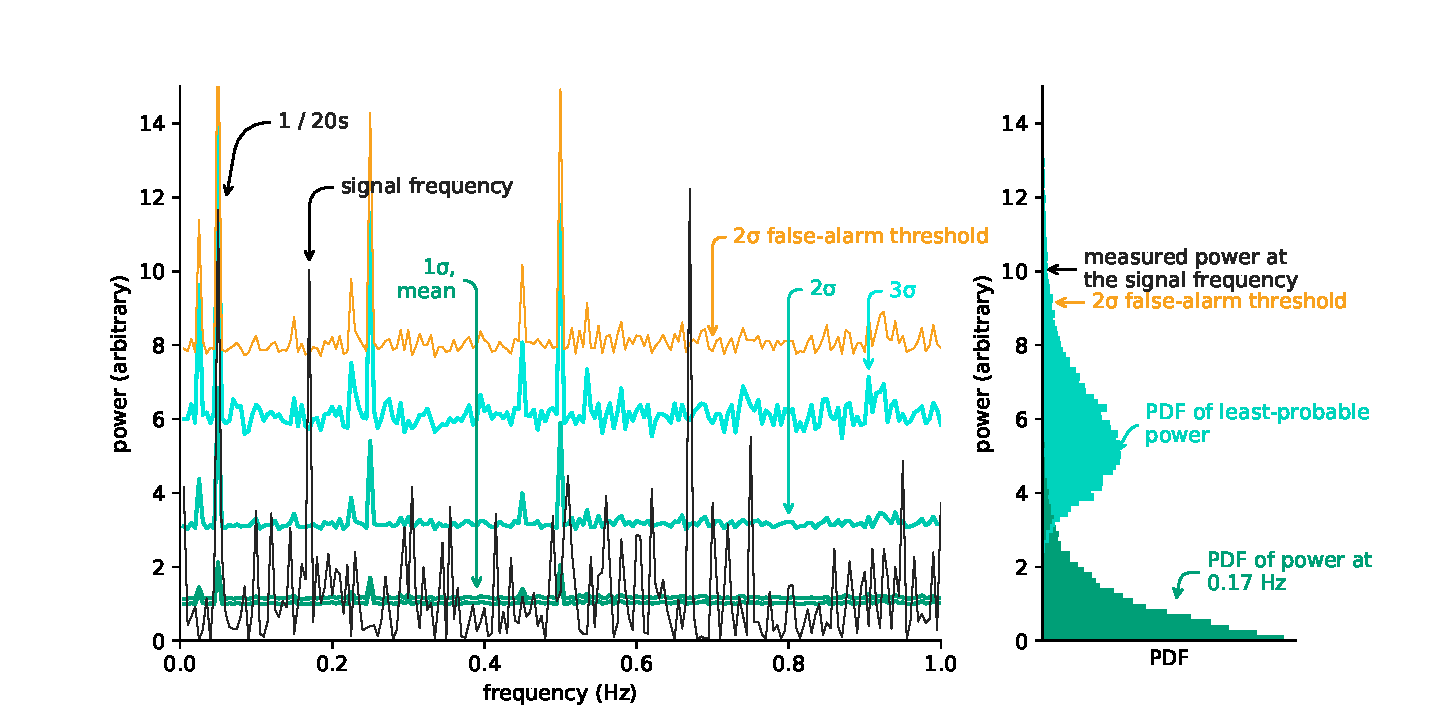
\includegraphics[width=.45\linewidth]{gfx/axions/basic_detection.pdf}}
%   \quad
%   \subfloat
%   % [The not--yet--real data tested against hypothetical signals using the \emph{CLs method}, in which hypotheses to which the experiment is not sensitive to get a statistical penalty. ]
%   {%\label{fig:basic_detection}
%   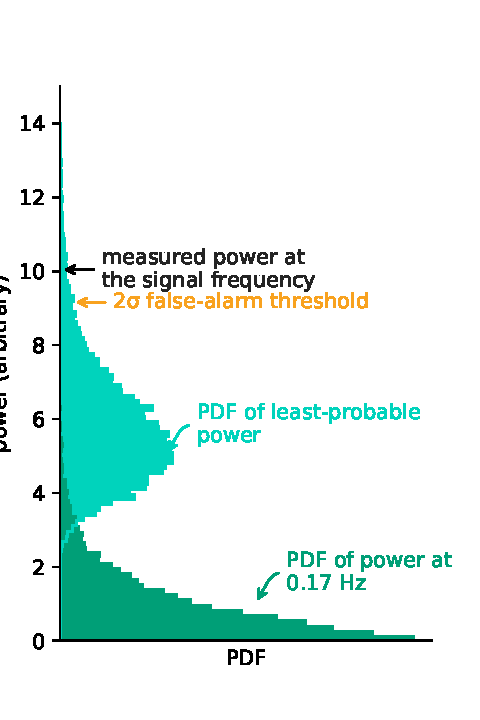
\includegraphics[width=.45\linewidth]{gfx/axions/basic_detection_histogram.pdf}}
%   \caption{Exclusion region --- signals that can be excluded at 95\% confidence level.}
%   \label{fig:basic_detection}
% \end{figure}

% It should be stressed that the distribution of $P_{max}$ is very different from the one of $P(\omega_{max})$. By looking for the highest peak, we check a big number of random variables $P(\omega_i)$ and pick a very special one --- the one that does lie the furthest in the tail of the distribution. The distribution of $P_{max}$ thus is centred around much higher values, as shown in Fig.\,\ref{fig:max_power_distribution}.

Let us now consider the local p-value of the most significant peak: $p_\text{min} \, | H_0$. If the points of the periodogram were perfectly uncorrelated, this would be a simple case of many hypothesis testing \cite{Algeri2016}. The CDF of the maximum of a set of uncorrelated variables is a product of their CDFs~\cite{Papoulis2002} and the local p-values $p_i$ are, by definition, uniformly distributed. So in this case we have
\begin{align}\label{eq:Fpmin}
  F_p(p) &= p \\
  F_{p_\text{max}}(p) &= p^N \\
  &\text{with}\ p' := 1 - p :\\
  F_{p_\text{min}}(p) &= 1 - F_{p'_\text{max}}(p') = 1 - (1 - p)^N \ ,
\end{align}
where $N$ is the number of frequencies tested.
% We Correlations in the periodogram, for example due to non-uniform sampling of the time-series, effectively lower $N$. If three dice are rolled in a way that two always give the same result, this is the same as rolling two dice when minimum roll is concerned.
The CDF of $p_\text{min} \, | H_0$, which we call $F^g$, can be estimated from the MC--generated data. Then the \emph{global} p-value is given by
\begin{equation}
  p^g = F^g(p_\text{min}^D) \ .
\end{equation}

We can further determine the global false-alarm thresholds. Traditionally, they are chosen to be at p-values of the normal distribution at integer multiples of its width $\upsigma$. The \emph{global} threshold p-value we call $p^g_{f.a.}$. The \emph{local} threshold p-value is:
\begin{equation}
  p_{f.a.} = \left( F^g \right)^{-1}(p^g_{f.a.}) \ .
\end{equation}
For each frequency the threshold power can be calculated according to the formula
\begin{equation}
  P^{f.a}_i = F_{P_i}^{-1}(1 - p_{f.a.}) \ .
\end{equation}
To claim a discovery of a significant oscillating signal, the false alarm probability has to be at most in the range of \num{2.87e-7}, the so-called 5$\upsigma$~\cite{PDG2016}. The false-alarm thresholds for toy time-series are depicted in Fig\,\ref{fig:basic_detection} in orange. They convey the intuitive massage: a single penetration of the 5$\upsigma$ false-alarm threshold anywhere would mean a 5$\upsigma$ confidence, that there is a statistically significant signal in the time-series.

In order to resolve the the tail of the CDF all the way down to 5$\upsigma$ false-alarm threshold, generating at least $10^8$ samples is necessary. Generic solutions of this problem are known (see for example section 39.3.2.2 \emph{The look-elsewhere effect} in \cite{PDG2016}). Here, a more specific approach is taken. We assume, that even though the CDF will deviate from the strictly derived equations in~\cite{Scargle1982}, the functional form of the tails will be preserved. Under the null hypothesis $F_{P_i}$ has the form $1 - e^{-P}$ \cite{Scargle1982}. For $F^g$ we assume a form of Eq.\,(\ref{eq:Fpmin}), where $N$ is a parameter that we have to fit to account for correlations in the periodogram. Those functional forms can be used to extrapolate tails of CDF estimated with much fewer MC samples.


% In Fig.\,\ref{fig:ILL_detection} we present the periodogram of a fake ILL dataset (geneated with the same run timings and uncertainties as in the real dataset, with run EDM values generated according to gaussian distribution with mean of $0$ and standard deviation equal to that run's uncertainty). We decided not to analyse the real data set until we are fully happy with the method.
%
% \begin{figure}[h!]
%   \begin{center}
%     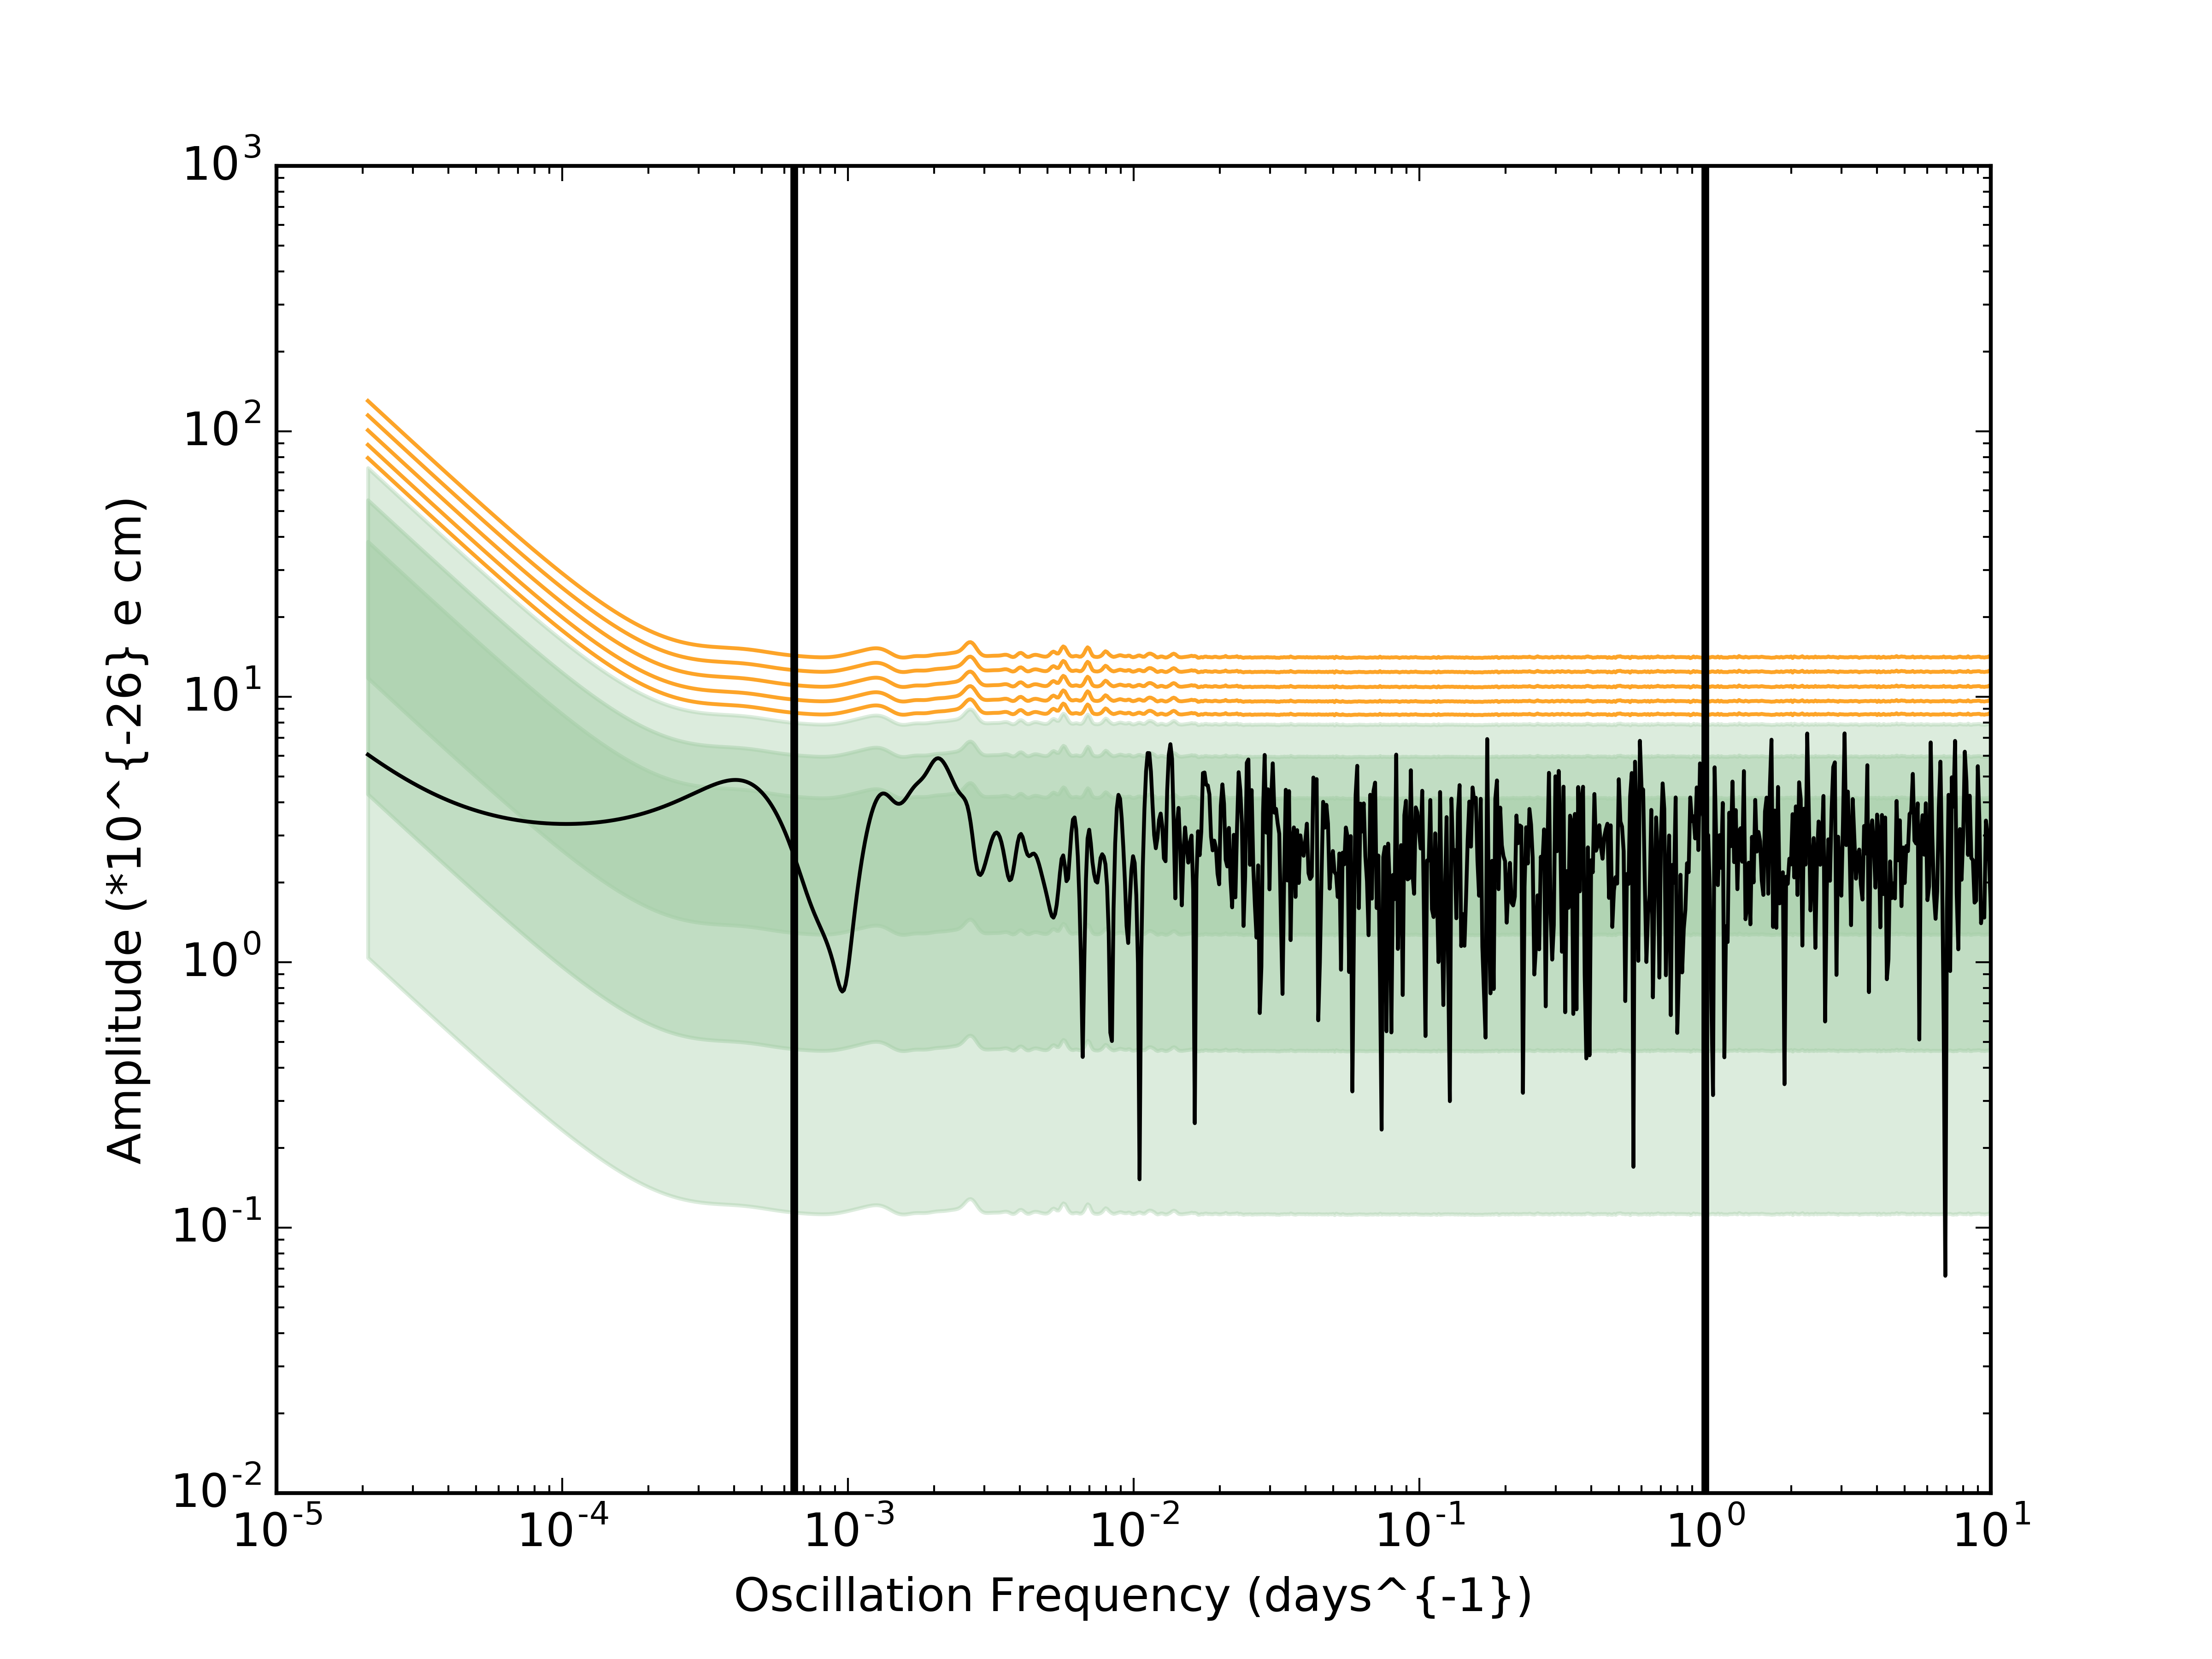
\includegraphics[width=\columnwidth]{gfx/axions/ILL_detection_Periodogram.png}
%     \caption{Periodogram of a fake ILL dataset. The green bands represent the distribution of the periodogram given the null hypothesis. The orange lines are 1-, 2-, 3-, 4-, 5--sigma false--alarm thresholds.}
%     \label{fig:ILL_detection}
%   \end{center}
% \end{figure}





\section{Signal hypotheses tests}
Should no claim for a discovery be possible, the next question to ask is:
\begin{center}
  \emph{Which oscillations would produce a visible peak, but did not, and can be thus excluded?}
\end{center}
In order to answer this question, the data need to be tested against being compatible with a number of model signal hypotheses. As an oscillation is characterised by its amplitude and frequency, the space of the hypotheses to test is two-dimensional.

\begin{figure}
  \centering 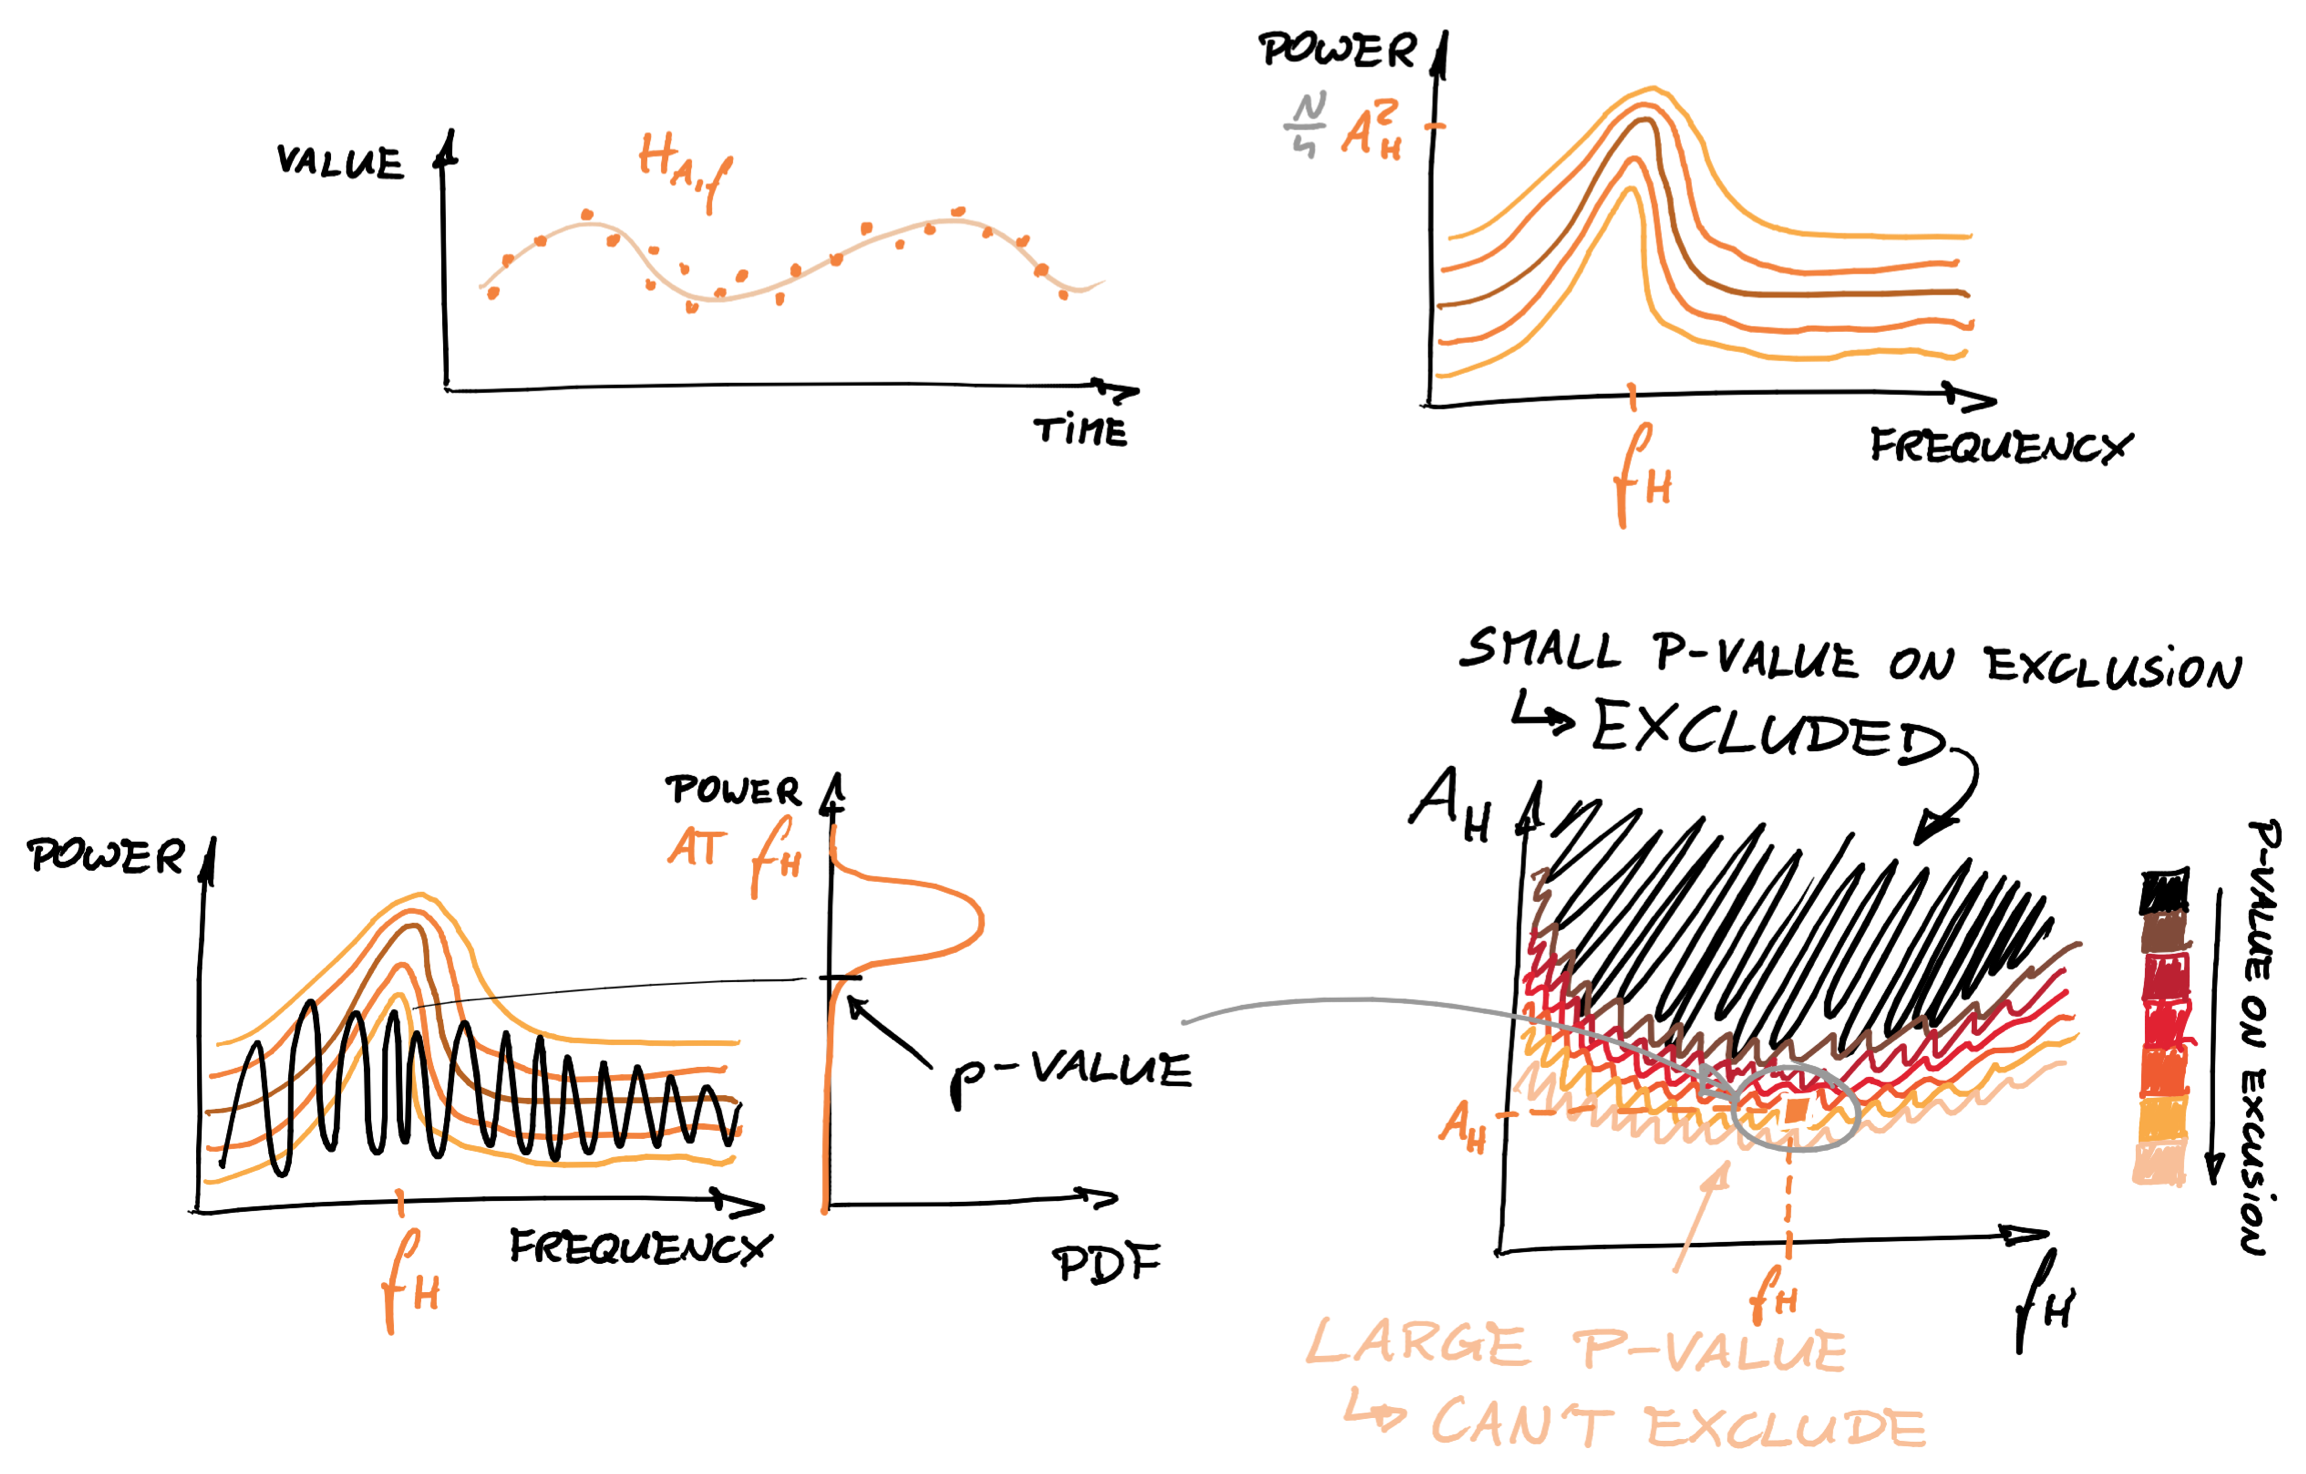
\includegraphics[width=\linewidth]{gfx/axions/exclusion_region.png}
  \caption{The general scheme for the determination of the exclusion region. First, a hypothesis about a signal, parametrised by its amplitude and frequency $f_H$, is assumed. Then, the distribution of the LSSA power at the freqeuncy $f_H$ is estimated under this assumption. The p-value of the time series' power, evaluated against the estimated distribution, is the measure of the confidence level on which the signal hypothesis can be rejected. This is repeated to cover the space of possible signals.}
  \label{fig:exclusion_region}
\end{figure}

The probability that a hypothetical oscillation of amplitude $A$ and frequency $\omega$ would produce less power at frequency $\omega$ then observed is
\begin{equation}
  % \mathrm{Pr}\left( P(\omega) < P^D(\omega)\ |\, H(\omega, A) \right) \ .
  \mathrm{Pr}\left( P^{H(\omega, A)}(\omega) < P^D(\omega)\ \right) \ .
\end{equation}
This probability is the p-value for the hypothesis $H(\omega, A)$ rejection. The distribution of $P^{H(\omega, A)}(\omega)$ is obtained with the Monte Carlo method. Here also the CDF's tail is extrapolated; this time, however, the one on the low-power side. We assume a functional form as eq.\,(15) in \cite{Scargle1982}. This test is repeated for different $\omega$ and $A$, each time covering a pixel of the space of possible hypotheses, as schematically shown in Fig.\,\ref{fig:exclusion_region}. The set of hypotheses excluded at most at certain p-value forms an exclusion region. We take the threshold p-value to be 5\%, which corresponds to the traditional confidence level of 95\%.

The frequency spectrum is covered much less densely than is the case in the null hypothesis test. This procedure is essentially evaluating the sensitivity of the measurement, which is solely determined by the timing and precision of the measurement points. No highly resonant structures are expected to appear therein. Also, a broader frequency range is covered, logarithmically spaced \SIrange[range-phrase=--,range-units=single]{e-3}{10}{\hertz}, in comparison to linearly spaced \SIrange[range-phrase=--,range-units=single]{5e-3}{1}{\hertz} in the test of the null hypothesis, in order to illustrate the behaviour of sensitivity of the method for extreme frequencies.

\marginpar{During the Monte Carlo simulations a perfectly coherent signal is assumed. The width of a real axion-induced peak is not resolvable by the nEDM experiment.}

% \begin{figure}
%   \myfloatalign
%   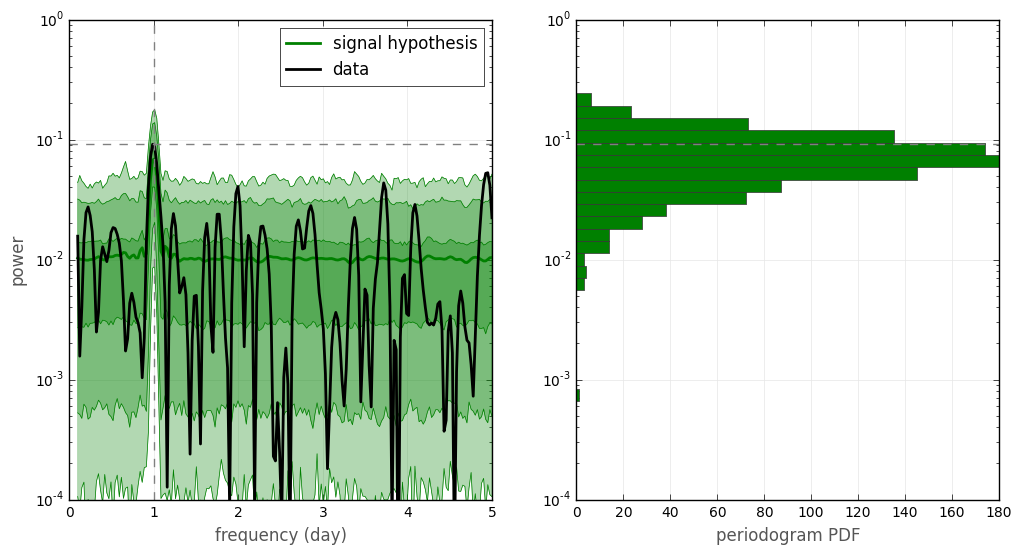
\includegraphics[width=.8\linewidth]{gfx/axions/axionMC_signal_hypothesis_rejection}
%   \caption
%   [...]
%   {
% \textsc{Left:} A periodogram of not--yet--real data on top of distribution of a periodogram of a hypothetical signal (green). \textsc{Right:} The distribution of power of the hypothetical signal at its model frequency.}
%   \label{fig:axions_signal_rejection}
% \end{figure}

\begin{figure}
  %FIXME directly copied from Elise's presentation on the 2015 PSI collaboration meeting
  \myfloatalign
  \subfloat
  [The test without the use of the CLs method.]
  % The white line connects points of 95\% C.L., surrounding an exclusion region. Note how deep into low amplitudes the line goes for couple of frequencies. See the text for the explanation. \note{Put a white line for the 95\% C.L. exclusion.}]
  {\label{fig:axions_exclusion_noCLs}
  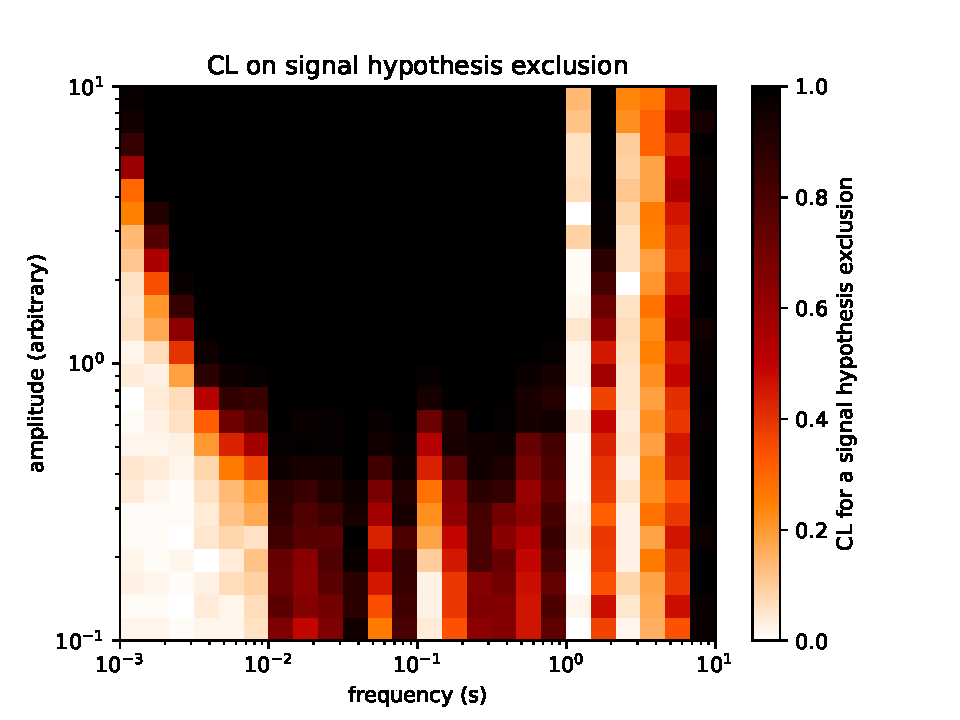
\includegraphics[width=.45\linewidth]{gfx/axions/basic_exclusion_noCls.pdf}}
  \quad
  \subfloat
  [The test with the use of the CLs method. Those hypotheses to which the measurement is not sensitive to get a statistical penalty.]
  {\label{fig:axions_exclusion_CLs}
  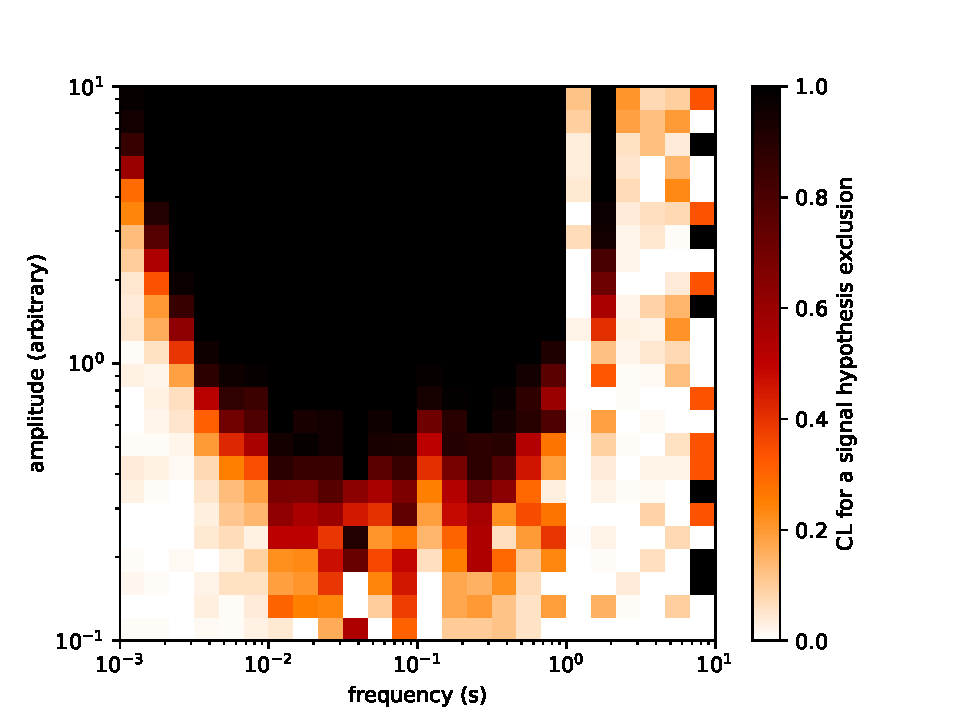
\includegraphics[width=.45\linewidth]{gfx/axions/basic_exclusion.pdf}}
  \caption{The toy time series tested against hypothetical signals. The signal space is spanned by their frequency and amplitude. The colour depicts the confidence level with which the signal can be rejected. The black region is excluded with a high confidence.}
  \label{fig:axions_exclusions}
\end{figure}

The result of this procedure applied to the toy time series (Fig.\,\ref{fig:basic_signal}) is presented on the left-hand side in Fig.\,\ref{fig:axions_exclusion_noCLs}. In the space of possible signals, the colour depicts the confidence level for rejecting the signals. The black region, corresponding to high confidence, is excluded. The region goes down to small amplitudes only in the region between \SI{e-2}{\hertz} (the time series is around \SI{200}{\second} long) and \SI{1}{\hertz} (a toy measurement was taken every 2 seconds).

\begin{figure}
  \centering 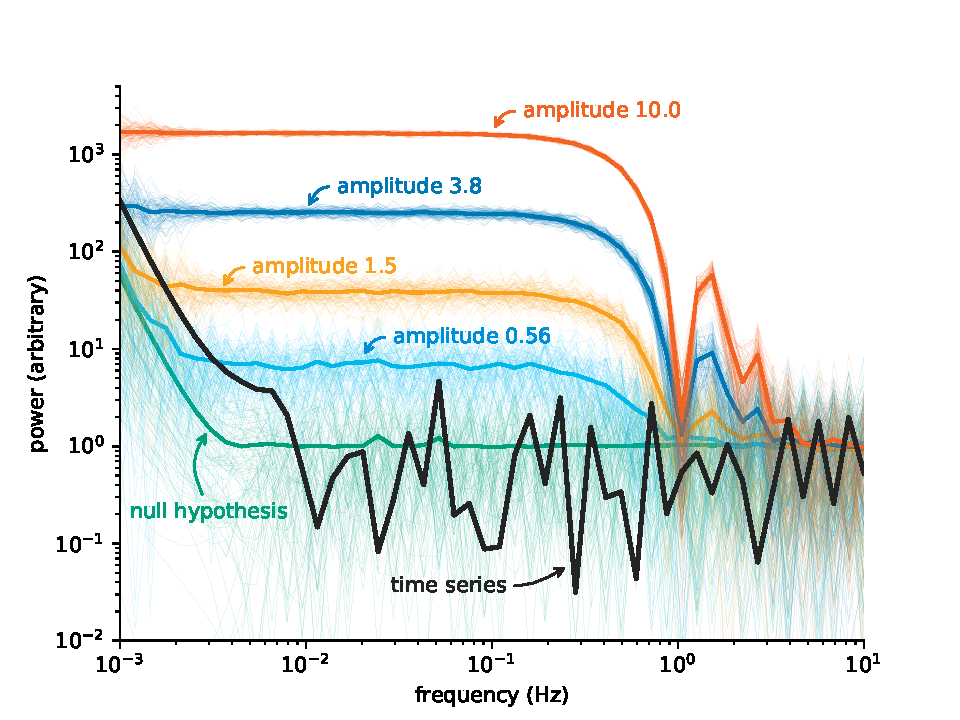
\includegraphics[width=0.8\linewidth]{gfx/axions/basic_exclusion_sensitivity.pdf}
  \caption{For each frequency, the LSSA power of a simulated signal of that frequency is plotted. Different colours correspond to different amplitudes of the signal, in particular no signal, the null hypothesis, is depicted in green. The lines has the interpretation of the height of a peak for different frequencies (the $x$ axis) and amplitudes (colours). The thin lines represent the different simulation outcomes, the thick ones---their average. The black line is the periodogram of the toy time series.}
  \label{fig:sensitivity}
\end{figure}

Why is the sensitivity constrained to this region can be understood by looking at Fig.\,\ref{fig:sensitivity}, where the average power obtained for various hypotheses is plotted together with the signal periodogram. Each coloured line depicts how high a signal peak would be, as the function of the frequency of the signal.
% For hypotheses with the same assumed amplitude of oscillation, the amplitude in the periodogram is constant for periods between the separation of the data points and the total length of the data set.
The signal peaks rise distinctly over the null hypothesis' periodogram only in a limited frequency range. Periods significantly longer than the length of the time series (below \SI{e-2}{\hertz}) are difficult to exclude, as it is always possible that the time series is located in an anti-node of an extremely slow oscillation. This manifests itself as a high amplitude seen even when the null hypothesis is assumed. On the other end, the power for frequencies above \SI{1}{\hertz} is suppressed, because the the measurements are not point-like, but rather the oscillation is averaged over a period of \SI{1}{\second}. There only little power arises, even for very large amplitudes of the signal.

% In particular, it is interesting to consider the difference between the 0 (offset) and the next frequency. Oscillations with a period longer than the span of the time series  appear in the series as a linear drift, if the measurements were taken in the linear part of the sine, or a quadratic change, if taken in the apex. Fitting such an oscillation is then equivalent to looking for a up--to--second--order drift in the data. Naturally, we expect the sensitivity to quickly worsen for these very long oscillations.

\begin{figure}
  \centering 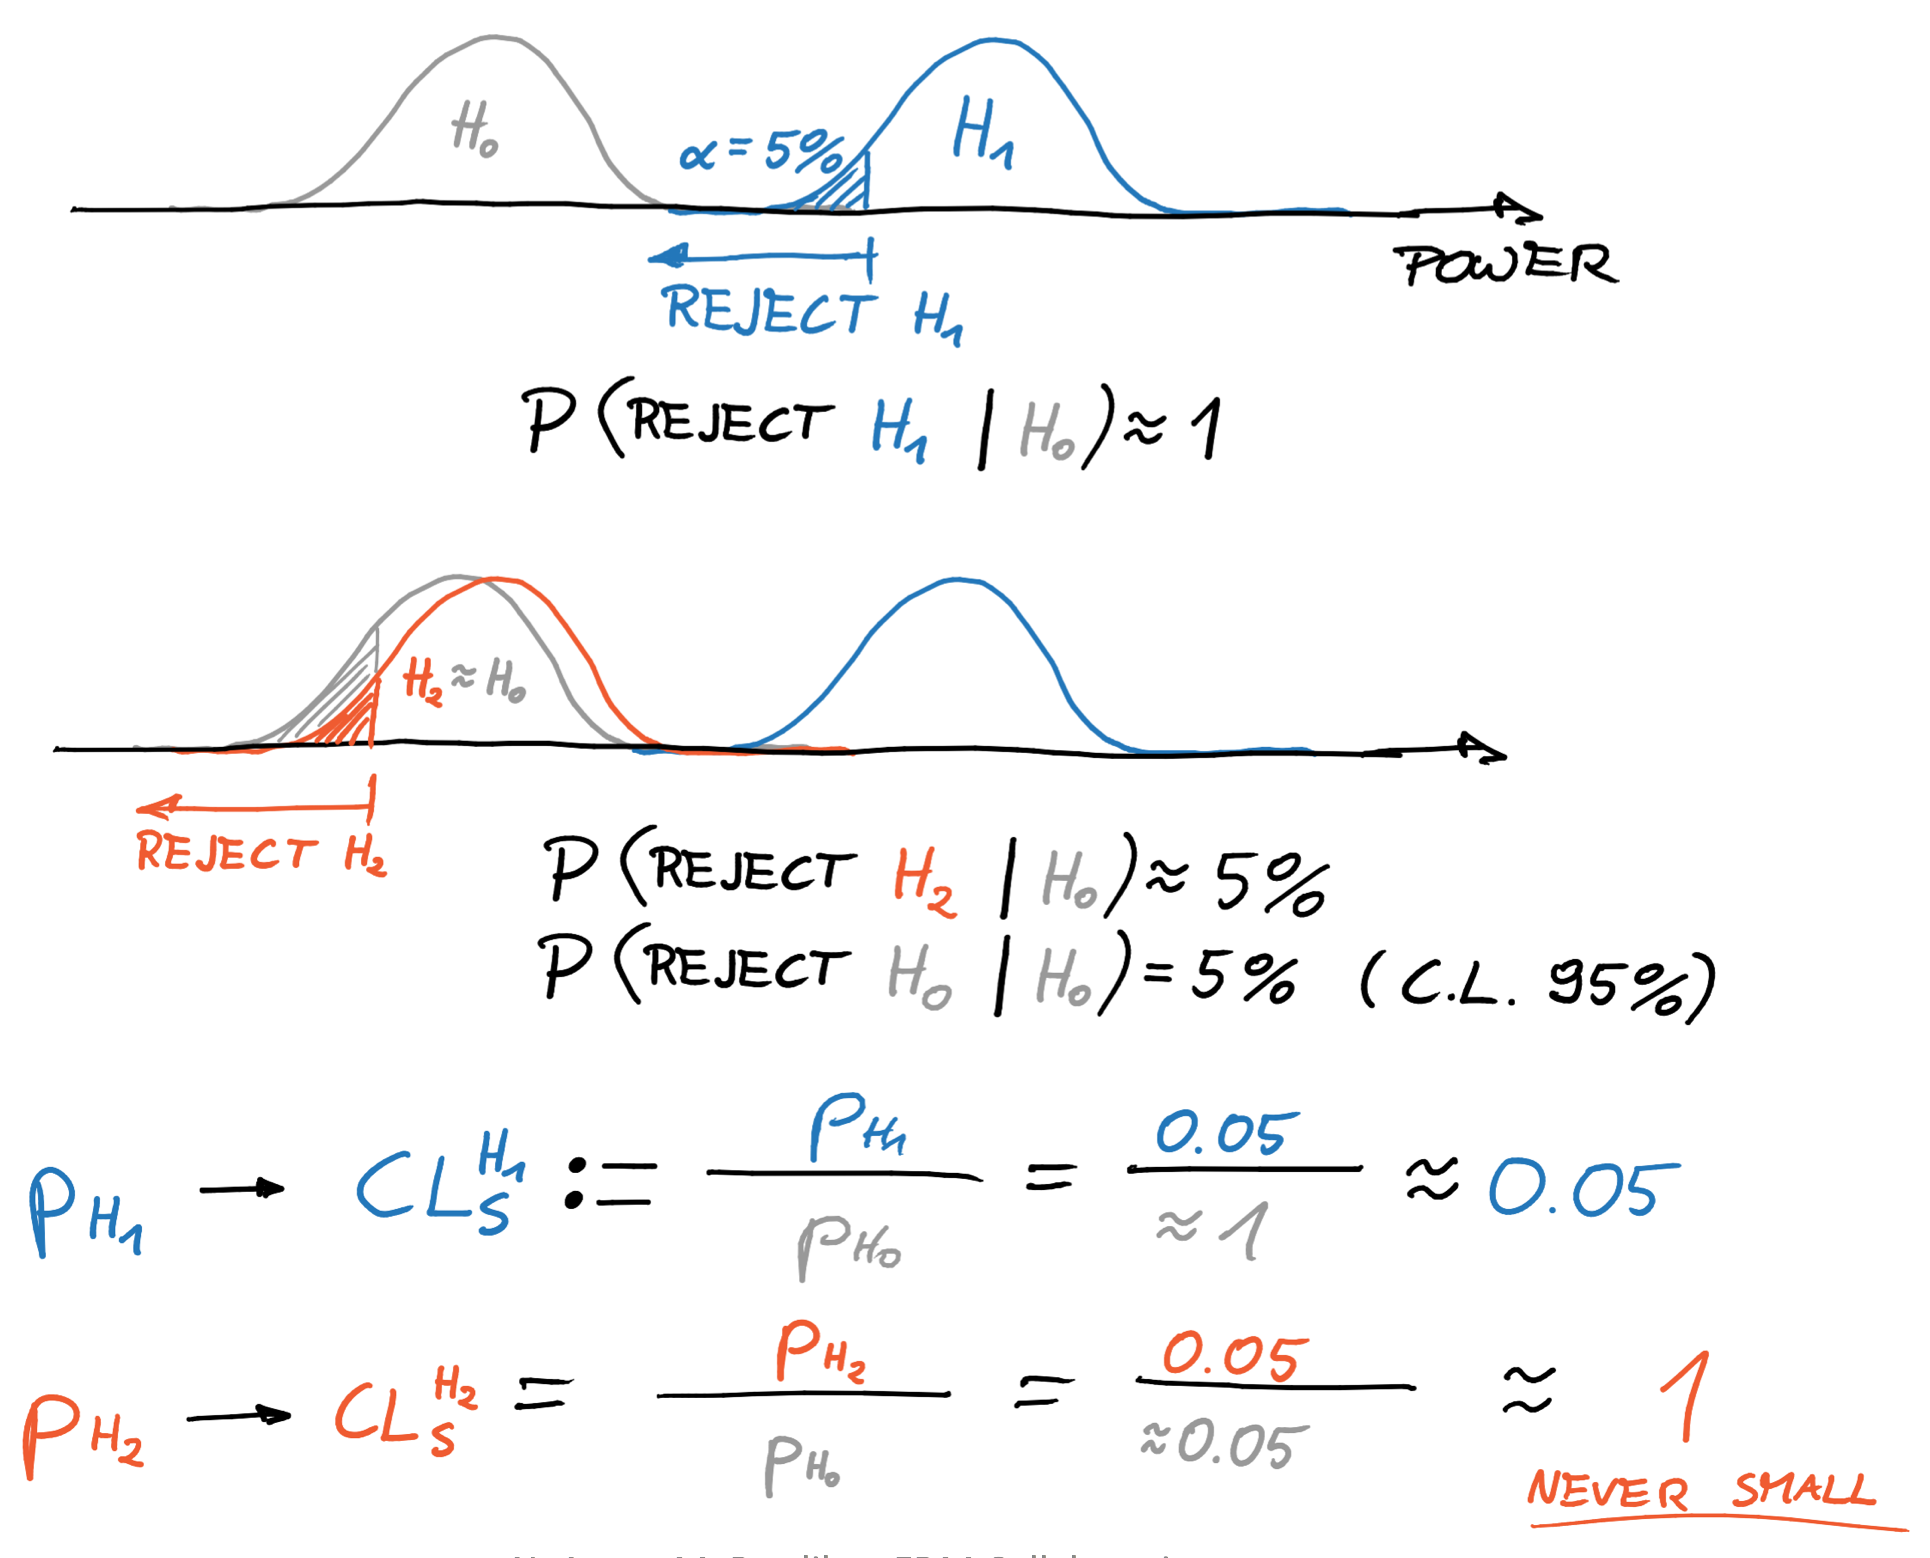
\includegraphics[width=0.7\linewidth]{gfx/axions/CLs.png}
  \caption{A graphical explanation of the motivation behind the CLs method. At the top: when the distributions of power for the null hypothesis $H_0$ and an alternative hypothesis $H_1$ are well separated, the probability of rejecting $H_1$ given $H_0$ is close to one. However, when we consider a signal of an arbitrarily small amplitude $H_2$, it still has roughly 5\% chance to be rejected, on a 95\% confidence level. If many of those are tested, 5\% will be unjustifiably rejected. In the CLs method one considers, rather then the p-value of an alternative hypothesis, the ratio of it to the p-value of the null hypothesis. This imposes a statistical penalty to the hypotheses not well separated from the null one.}
  \label{fig:CLs}
\end{figure}

The black exclusion region in Fig.\,\ref{fig:axions_exclusion_noCLs} exhibits a number of thin peaks going down to very low amplitudes. Seemingly, for some frequencies, even tiny signals can be confidently excluded. This is rightfully disturbing. Consider, however, that as the power was evaluated for many frequencies, inevitably at some of them, roughly 5\%, the power is low enough to be rejected at 95\% confidence level, even when tested against the distribution of power given the null hypothesis itself. It is completely fine from the statistical point of view, yet physicists prefer not to allow a situation, where a hypothesis is rejected based on a measurement which was not sensitive to it. One possible solution is called the \emph{CLs method}. The method is defined, as well as the problem itself discussed, in the booklet of the Particle Data Group~\citep{PDG2016}. A short graphical explanation can be found in Fig.\,\ref{fig:CLs}. With use of the CLs method the exclusion is suppressed in the region of low sensitivity, as shown on the right-hand side in Fig.\,\ref{fig:axions_exclusion_CLs}.

Calculating each pixel of the alternative hypotheses space may be considered as largely a waste of resources. Rather than covering the whole space, one may resolve only only the 95\% C.L. threshold. This can be done, for example with the bisection algorithm run at each frequency. In this case only 10 steps gave a relative precision below 0.01 on the threshold's position.

In this chapter the least squares spectral analysis, LSSA, has been introduced as a method to look for oscillations in unevenly sampled time series with unequal error bars. The test of the null hypothesis, no signal present, gives the estimate of the level of confidence, on which a discovery of an oscillating signal can be claimed. Then, a space possible signals is explored to determine, which ones can be excluded on the ground of not having been detected. In the next chapter this methodology is applied to the time series of the neutron electric dipole moment measurements performed in PSI. An oscillation there would be a hint for an axion dark matter.
